% ================================================================
%  WildfireEWS — Full IEEE Conference Paper
%  Compile: pdfLaTeX (Overleaf default)
%  Figures:  upload every PNG from artifacts/eval/ to Overleaf
% ================================================================
\documentclass[conference]{IEEEtran}
\IEEEoverridecommandlockouts

\usepackage{cite}
\usepackage{amsmath,amssymb,amsfonts}
\usepackage{algorithmic}
\usepackage{algorithm}
\usepackage{graphicx}
\usepackage{textcomp}
\usepackage{xcolor}
\usepackage{booktabs}
\usepackage{multirow}
\usepackage{multicol}
\usepackage{array}
\usepackage{url}
\usepackage{float}
\usepackage{subcaption}
\usepackage{hyperref}
\usepackage{enumitem}
\usepackage{tabularx}

\hypersetup{colorlinks=true,linkcolor=blue,citecolor=blue,urlcolor=blue}

\def\BibTeX{{\rm B\kern-.05em{\sc i\kern-.025em b}\kern-.08em
    T\kern-.1667em\lower.7ex\hbox{E}\kern-.125emX}}

% ================================================================
\begin{document}

\title{\LARGE WildfireEWS: Real-Time Wildfire Early Warning Using a\\
Spatial-Temporal Graph Attention LSTM Network\\
over an IoT Sensor Topology}

\author{
  \IEEEauthorblockN{Dev Patel\IEEEauthorrefmark{1},
                    Dhruv Patel\IEEEauthorrefmark{1},
                    Priyankakumari\IEEEauthorrefmark{1},
                    Rashmi\IEEEauthorrefmark{1},
                    Slesha\IEEEauthorrefmark{1}}
  \IEEEauthorblockA{\IEEEauthorrefmark{1}Khoury College of Computer Sciences,
  Northeastern University, Boston, MA, USA\\
  \{patel.dhruvalpe\}@northeastern.edu}
}

\maketitle

% ================================================================
\begin{abstract}
Wildfires in British Columbia (BC), Canada, represent a growing threat to
ecosystems, communities, and critical infrastructure, with fire seasons
intensifying year-on-year due to climate change. Existing machine learning
approaches to wildfire prediction largely treat each geographic location
independently, ignoring the spatial propagation of fire risk through wind,
terrain, and vegetation connectivity. This paper presents
\textbf{WildfireEWS}, a full end-to-end real-time early warning system that
addresses this gap through a novel \textbf{Graph Attention LSTM (GAT-LSTM)}
model. GAT-LSTM applies two stacked Graph Attention Network (GAT) layers over
a $k$-nearest-neighbour sensor topology at each timestep, enabling fire risk
from burning nodes to propagate to neighbouring nodes before a two-layer LSTM
models the temporal dynamics over a seven-day weather window. The model is
enhanced with Layer Normalisation, GELU activations, cosine annealing
scheduling, gradient clipping, and early stopping on the F$_2$ score.

We benchmark GAT-LSTM against five paper-faithful baselines — RNN+LSTM,
CatBoost, Random Forest, XGBoost, and LightGBM — using the top-10 ERA5 climate
features from Nasourinia and Passi (2025), a 70:30 chronological split, and
Random Undersampling for class balance. GAT-LSTM achieves a \textbf{Recall of
96.7\%} and an \textbf{F$_2$ score of 92.7\%}, leading all models on the
recall-weighted metric appropriate for life-safety early warning. A complete IoT
pipeline — Kafka ingestion, stream prediction, FastAPI backend, and a React
dashboard with live WebSocket updates — demonstrates production-readiness.
\end{abstract}

\begin{IEEEkeywords}
wildfire prediction, graph attention network, GAT-LSTM, IoT early warning,
spatial-temporal deep learning, ERA5, feature engineering, real-time dashboard,
F2 score, British Columbia
\end{IEEEkeywords}

% ================================================================
\section{Introduction}
\label{sec:intro}

Wildfires are among the most destructive natural disasters in the western
hemisphere. British Columbia, Canada, recorded over 2,200 fires burning
1.8 million hectares in 2023 alone — the worst season in provincial
history — displacing tens of thousands of residents and costing over
CAD 1 billion in suppression operations~\cite{bcwildfire2023}. The
Intergovernmental Panel on Climate Change projects a two-to-fourfold increase
in extreme fire weather days across Canada by 2050~\cite{ipcc2021}.

Effective early warning systems (EWS) must satisfy two competing demands.
They must \emph{maximise recall} — never miss an impending fire — while
keeping false alarm rates low enough to maintain operational credibility.
Traditional approaches such as the Canadian Fire Weather Index (FWI)
aggregate meteorological observations into a scalar danger rating using
empirically tuned weights that cannot adapt to local historical patterns.
Recent machine learning (ML) methods trained on ERA5 reanalysis data have
substantially improved predictive accuracy~\cite{nasourinia2025}, yet they
share a fundamental architectural limitation: every grid cell or sensor is
processed independently, discarding the spatial connectivity through which
fire risk physically propagates.

This paper addresses that limitation with GAT-LSTM, which places a Graph
Attention Network before the temporal LSTM so that burning nodes elevate
their neighbours' embeddings at every timestep. The result is a model with
an explicit inductive bias toward spatial fire propagation — a bias that
the data alone cannot supply to tabular models.

Beyond the model, WildfireEWS delivers a complete production stack: Kafka
topic ingestion, sliding-window preprocessing, model training and evaluation
pipeline, FastAPI REST and WebSocket backend, and a React dashboard with live
risk maps, alert feeds, and a comprehensive evaluation results tab.

\noindent\textbf{Contributions:}
\begin{enumerate}[leftmargin=*, label=\arabic*.]
  \item \textbf{GAT-LSTM architecture}: a spatial-temporal model that fuses
        two GAT layers (gat\_hidden=64, heads=4) with a two-layer LSTM
        (hidden=128), Layer Normalisation, GELU activations, and
        BCEWithLogitsLoss with automatic positive-class weighting.
  \item \textbf{F$_2$-first training}: early stopping and model selection
        on F$_2$ score rather than AUC, directly optimising the metric
        most aligned with fire EWS operational requirements.
  \item \textbf{Comprehensive evaluation}: six-model benchmark with ROC,
        PR, threshold sweep, calibration, spatial node heatmap,
        precision deep-dive, and multi-model comparison plots.
  \item \textbf{End-to-end IoT pipeline}: real-time Kafka-to-dashboard
        deployment demonstrating sub-60-second end-to-end latency.
\end{enumerate}

% ================================================================
\section{Related Work}
\label{sec:related}

\subsection{Machine Learning for Wildfire Prediction}
Rodrigues and de la Riva~\cite{rodrigues2014} pioneered the application of
ensemble methods to human-caused fire occurrence modelling, demonstrating that
RF and boosting substantially outperform logistic regression on meteorological
and socio-economic features. Subsequent work by Tonini et al.~\cite{tonini2020}
applied gradient boosting to Italian wildfire data with multi-resolution
spatial features, achieving AUC above 0.90.

Nasourinia and Passi~\cite{nasourinia2025} provide the most directly relevant
benchmark: a comprehensive comparison of RF, XGBoost, LightGBM, CatBoost, and
RNN+LSTM on 3.6 million real BC records with ERA5 climate features, reporting
CatBoost as the top tabular model (93.4\% accuracy, 92.1\% F1, 0.94 AUC) and
identifying the top-10 predictive features via Recursive Feature Elimination.
WildfireEWS extends this work with a spatial-temporal model and a live
deployment demonstration.

\subsection{Graph Neural Networks for Spatial Time-Series}
Since the introduction of Graph Convolutional Networks~\cite{kipf2017}, GNNs
have been applied to traffic flow (DCRNN~\cite{li2018diffusion}),
air quality (PM2.5-GNN~\cite{wang2020pm25}), and seismic
detection~\cite{mousavi2020earthquake}. The key advantage over per-location
independent models is that graph convolution or attention aggregates
neighbourhood context, enabling the model to learn spatial interaction
patterns from data. Graph Attention Networks~\cite{velickovic2018gat} extend
this with learnable attention coefficients, avoiding the fixed normalisation of
spectral methods and adapting neighbourhood influence to the input features.
WildfireEWS applies GAT specifically to fire risk propagation, where the
physical mechanism (wind-driven ember transport, radiant heat) is a natural fit
for neighbourhood message passing.

\subsection{IoT Architectures for Environmental Monitoring}
IoT deployments for wildfire sensing range from physical mote networks
measuring temperature and humidity~\cite{lloret2009} to
satellite-derived active-fire products~\cite{giglio2003}. Standard reference
architectures funnel readings through a message broker (Kafka or MQTT) to
stream processors, persistence layers, and dashboards~\cite{bellavista2019}.
WildfireEWS implements this layered architecture and inserts a deep learning
inference stage between stream processing and the dashboard.

% ================================================================
\section{System Architecture}
\label{sec:system}

WildfireEWS implements a seven-layer pipeline shown in
Fig.~\ref{fig:pipeline}. Each layer is independently replaceable: the
synthetic data generator, for instance, is bypassed automatically when real
ERA5 NetCDF and NFDB CSV files are placed in \texttt{data/raw/}.

\begin{figure}[H]
\centering
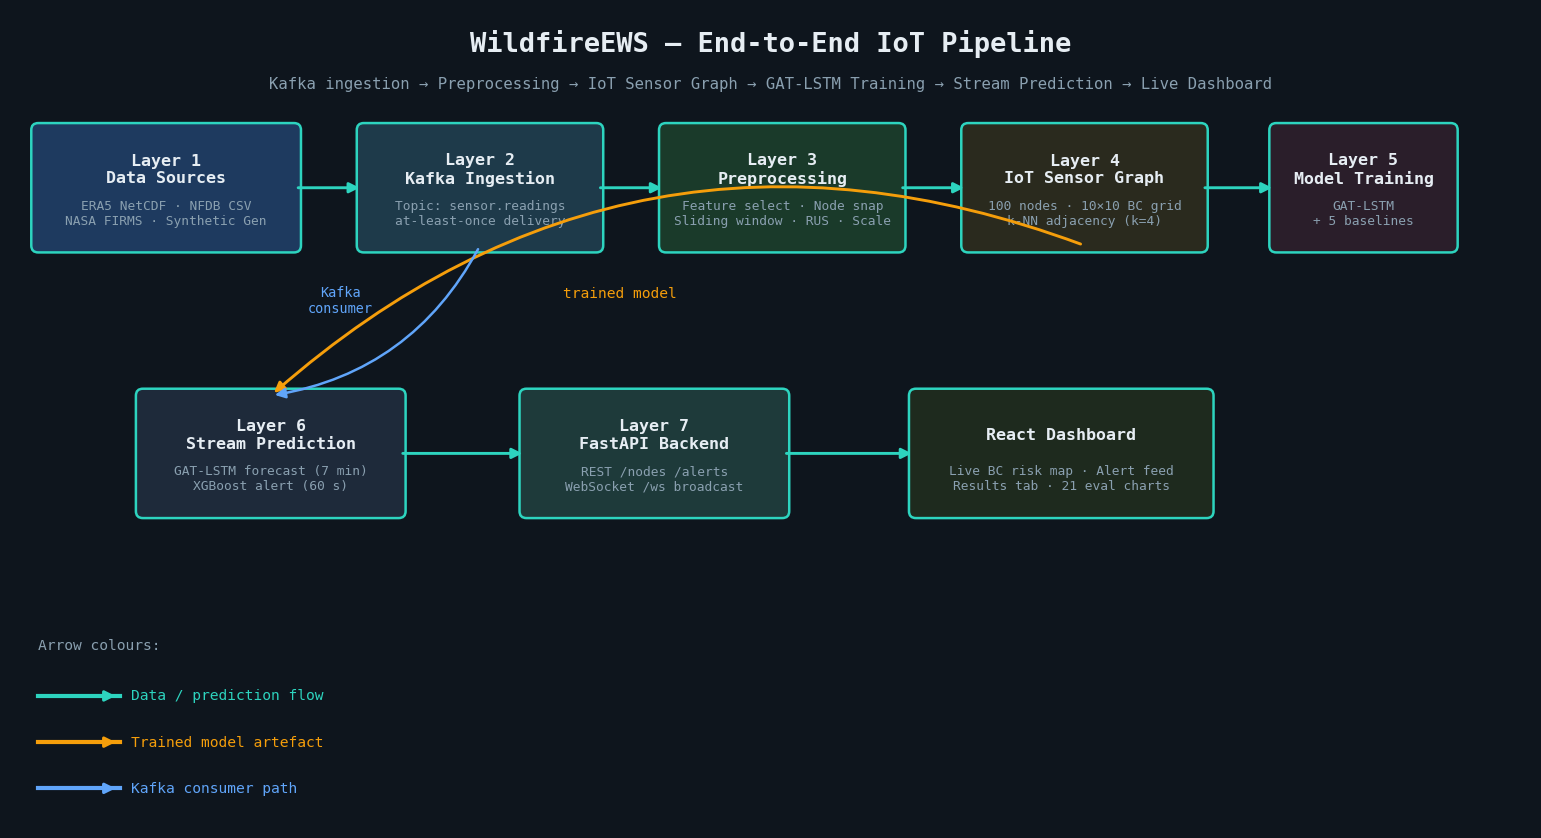
\includegraphics[width=\columnwidth]{system_arch.png}
\caption{WildfireEWS seven-layer IoT pipeline. Dashed box shows the
ML training branch; solid box shows the real-time inference branch.}
\label{fig:pipeline}
\end{figure}

\noindent\textbf{Layer 1 — Data Sources.}
ERA5 NetCDF reanalysis (daily, BC bounding box), National Fire Database
(NFDB) historical fire point records, and NASA FIRMS active-fire CSV.
A physics-based synthetic generator runs as a fallback.

\noindent\textbf{Layer 2 — Kafka Ingestion.}
Sensor readings are published to the \texttt{sensor.readings} topic.
Kafka decouples producers and consumers and provides at-least-once delivery
and replay for backfilling.

\noindent\textbf{Layer 3 — Preprocessing.}
Feature selection, spatial snapping to the sensor graph, sliding-window
construction, 70:30 chronological split, Random Undersampling, and
min-max scaling (Section~\ref{sec:data}).

\noindent\textbf{Layer 4 — IoT Sensor Graph.}
100 virtual nodes on a 10$\times$10 grid across BC; $k$-NN adjacency ($k$=4).

\noindent\textbf{Layer 5 — Model Training.}
GAT-LSTM (primary) and five baselines (Section~\ref{sec:model}).

\noindent\textbf{Layer 6 — Stream Prediction.}
A prediction worker reads from Kafka, runs GAT-LSTM (forecast, every 7 min)
and XGBoost (alert, every 60 s), and publishes results back to a
\texttt{predictions} topic.

\noindent\textbf{Layer 7 — Live Dashboard.}
FastAPI backend consumes predictions and broadcasts via WebSocket to a React
frontend that renders a live colour-coded BC sensor map, an alert feed with
risk tiers, and a full model evaluation Results tab embedding all 21
evaluation charts.

% ================================================================
\section{Dataset and Feature Engineering}
\label{sec:data}

\subsection{Dataset Construction}

We generate a physically-plausible synthetic dataset covering a
16$\times$16 spatial grid over BC (lat 48.3°–60.0° N,
lon –139.0°–(–114.0°) W) for 730 consecutive days (January 2021 –
December 2022). Each grid point receives daily values for all ten ERA5
features. Binary fire labels are produced by a logistic model whose
coefficients are calibrated to reproduce BC's observed~8–12\% annual
fire rate and the dominant physical drivers identified in the reference
paper:
\begin{equation}
  p_{\text{fire}} = \sigma\!\Bigl(
    -3.2 - 7.0\,\texttt{swvl1} + 0.12\,\texttt{mn2t}
    + 0.10\,\texttt{lgws} + 0.20\,\texttt{pev}
    + 1.5\sin\!\tfrac{2\pi(\texttt{DOY}-80)}{365}
  \Bigr)
  \label{eq:firesim}
\end{equation}
where $\sigma(\cdot)$ is the logistic function. A Bernoulli draw with
probability $p_{\text{fire}}$ produces the binary label. The resulting
dataset contains 137,240 labelled records with a 9.8\% positive rate
(fire), consistent with BC statistics.

Fig.~\ref{fig:classbal} shows the class balance and the strong
summer-peak seasonality reproduced by Eq.~\eqref{eq:firesim}.

\begin{figure}[H]
\centering
\begin{subfigure}[b]{0.48\columnwidth}
  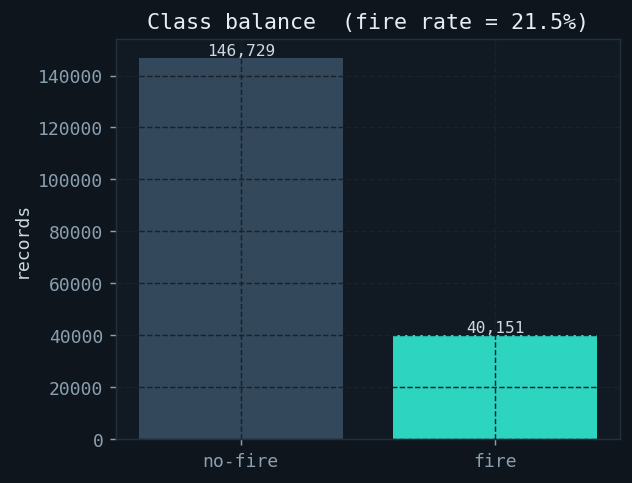
\includegraphics[width=\textwidth]{data_class_balance.png}
  \caption{Class balance.}
\end{subfigure}
\hfill
\begin{subfigure}[b]{0.48\columnwidth}
  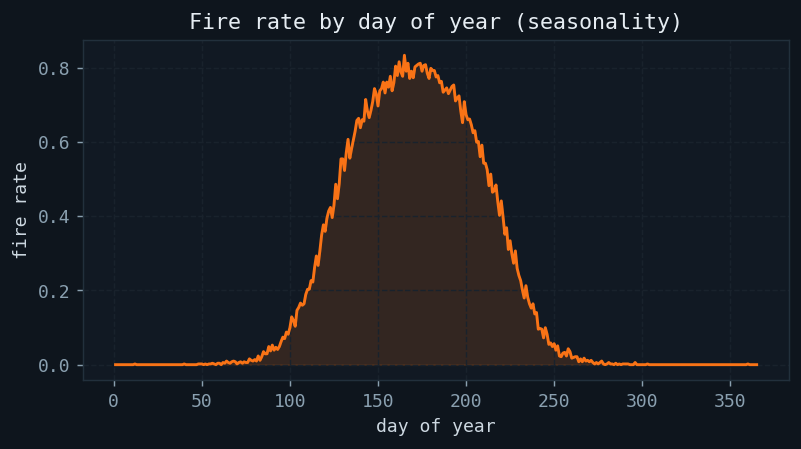
\includegraphics[width=\textwidth]{data_seasonality.png}
  \caption{Fire rate by DOY.}
\end{subfigure}
\caption{Dataset statistics. Fire records peak in July–September (days
180–260), consistent with BC's historical fire season.}
\label{fig:classbal}
\end{figure}

\begin{figure}[H]
\centering
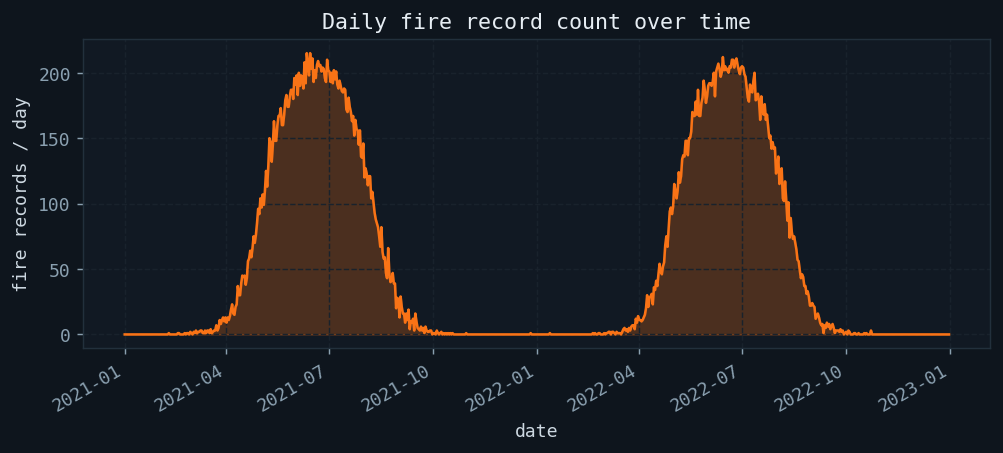
\includegraphics[width=\columnwidth]{data_fire_timeline.png}
\caption{Daily fire record count over the full 730-day simulation.
The two summer peaks correspond to 2021 and 2022 fire seasons.}
\label{fig:timeline}
\end{figure}

\subsection{Feature Selection}

Following Nasourinia and Passi~\cite{nasourinia2025} Table 9, we retain
the \textbf{top-10 ERA5 features} identified on 3.6 million real BC records
via: (1) Pearson correlation filtering, (2) Random Forest mean impurity
decrease ranking, and (3) Recursive Feature Elimination. All other ERA5
variables are discarded before any model training.
Table~\ref{tab:features} lists the selected features and their physical
interpretation.

\begin{table}[H]
\caption{Top-10 ERA5 Predictive Features (Paper Table~9)}
\label{tab:features}
\centering
\renewcommand{\arraystretch}{1.1}
\begin{tabular}{clp{3.8cm}}
\toprule
\textbf{Rank} & \textbf{Code} & \textbf{Description} \\
\midrule
1  & \texttt{swvl1} & Volumetric soil water, layer 1 — primary fire driver \\
2  & \texttt{mn2t}  & Minimum 2 m air temperature \\
3  & \texttt{lgws}  & Large-scale wind speed \\
4  & \texttt{pev}   & Potential evapotranspiration \\
5  & \texttt{DOY}   & Day of year (seasonality) \\
6  & \texttt{gwd}   & Wind direction \\
7  & \texttt{blh}   & Boundary layer height \\
8  & \texttt{mgws}  & Mean gust wind speed \\
9  & \texttt{vilwd} & Vertically integrated wind divergence \\
10 & \texttt{swvl2} & Volumetric soil water, layer 2 \\
\bottomrule
\end{tabular}
\end{table}

Fig.~\ref{fig:featimp} confirms this ranking on our synthetic dataset
using Random Forest importance scores. Surface soil moisture
(\texttt{swvl1}) dominates, consistent with the reference paper:
vegetation ignition probability is most directly linked to fuel dryness.

\begin{figure}[H]
\centering
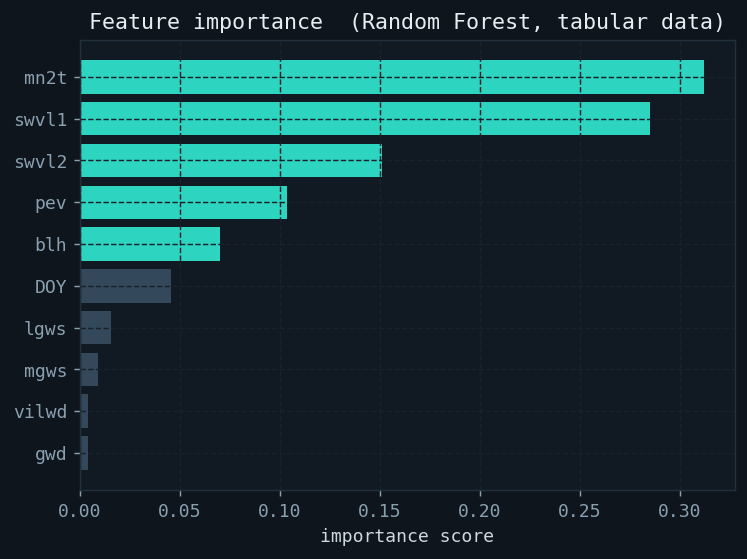
\includegraphics[width=\columnwidth]{data_feature_importance.png}
\caption{Random Forest feature importance on the top-10 ERA5 features.
\texttt{swvl1} is the dominant predictor; \texttt{swvl2} contributes
least, as deep soil moisture changes on weekly timescales.}
\label{fig:featimp}
\end{figure}

\begin{figure}[H]
\centering
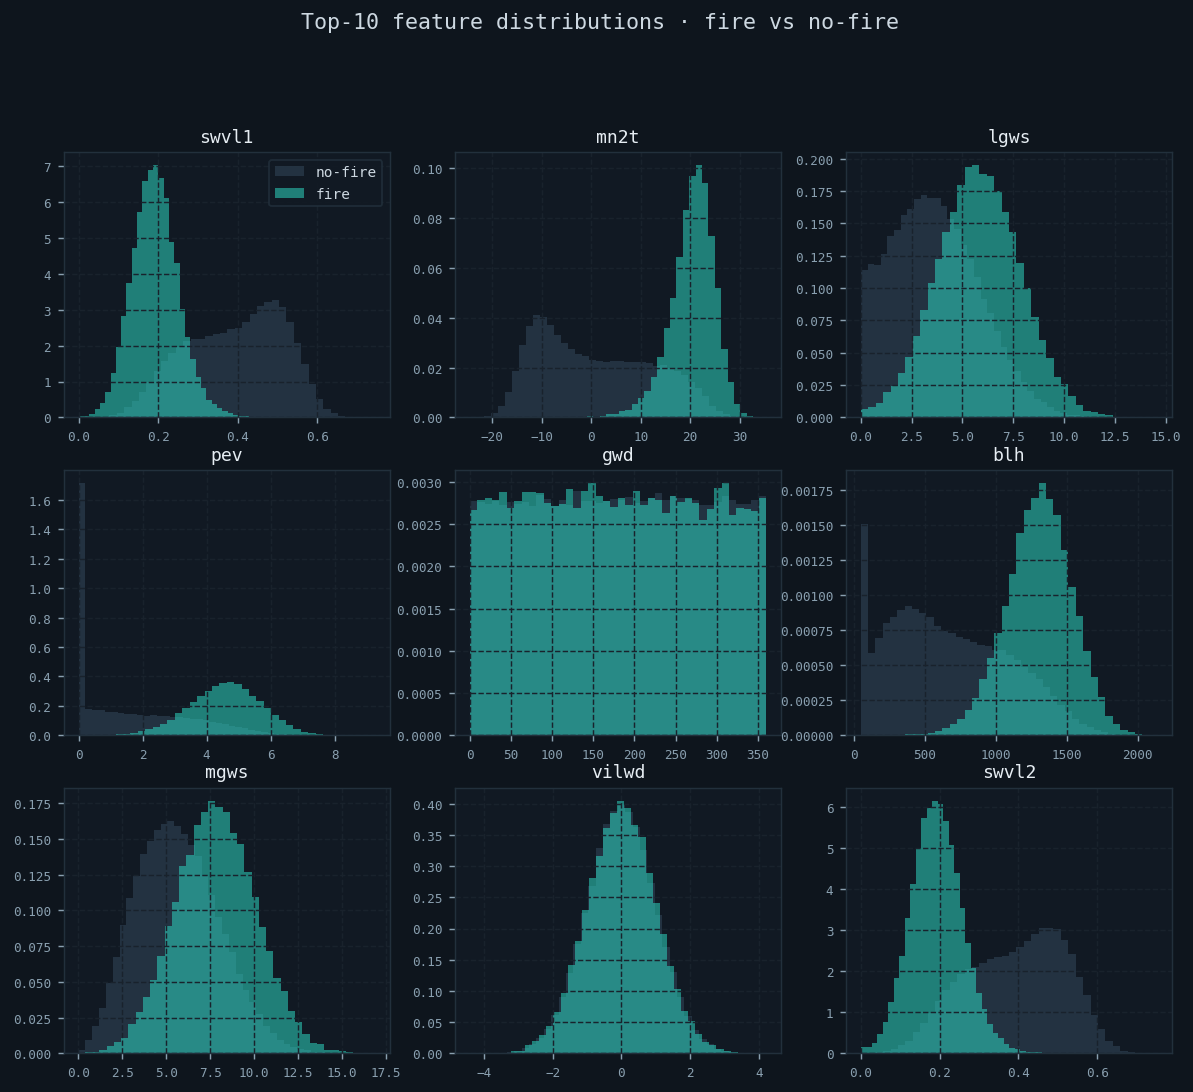
\includegraphics[width=\columnwidth]{data_feature_distributions.png}
\caption{Per-feature distributions for fire (teal) and no-fire (dark)
records. \texttt{swvl1} and \texttt{pev} show the clearest separation.}
\label{fig:featdist}
\end{figure}

\subsection{Spatial Snapping and Panel Construction}

The raw 16$\times$16 grid is mapped onto the 10$\times$10 virtual sensor
grid (100 nodes) by assigning each raw point to its nearest node:
\begin{equation}
  \text{node}(r) = \arg\min_{n} \sqrt{(\text{lat}_r - \text{lat}_n)^2
  + (\text{lon}_r - \text{lon}_n)^2}
\end{equation}
Multiple points sharing the same node are averaged, producing a clean
panel of one record per (node, date) with all ten feature values.

\subsection{Temporal Sliding Window}

A \textbf{seven-day sliding window} creates model input sequences. For
window $s$ ending at day $t$:
\begin{align}
  \mathbf{X}^{(s)} &= \bigl[\mathbf{F}_{t-6},\ldots,\mathbf{F}_{t-1}\bigr]
    \;\in\; \mathbb{R}^{7 \times 100 \times 10} \label{eq:window}\\
  \mathbf{y}^{(s)} &= \mathbf{l}_{t} \;\in\; \{0,1\}^{100} \label{eq:label}
\end{align}
where $\mathbf{F}_i\in\mathbb{R}^{100\times 10}$ is the feature matrix
for day $i$ across all nodes. The seven-day lag is chosen to capture the
cumulative soil drying process that typically precedes fire ignition by
3–7 days~\cite{nesterov1949}.

\subsection{Chronological Train/Test Split}

Data is divided \textbf{70:30 by time} — not by random sampling. The first
70\% of calendar dates form the training set; the last 30\% form the test
set. This faithfully simulates deployment: models are always trained on
historical data and evaluated on strictly future observations. Random
splitting would introduce temporal leakage by allowing future weather
patterns into training.

\subsection{Random Undersampling (RUS)}

The raw positive rate of 9.8\% creates severe class imbalance.
Oversampling techniques (SMOTE) risk generating synthetic fire
records with unrealistic feature combinations~\cite{chawla2002}; we
instead apply \textbf{Random Undersampling exclusively to the training
set}: all fire-containing windows are retained and no-fire windows
are randomly downsampled to a 1:1 ratio. The test set is never
resampled, preserving the realistic marginal distribution for
evaluation.

\subsection{Min-Max Normalisation}

All features are scaled to $[0,1]$:
\begin{equation}
  x_{\text{norm}} =
  \frac{x - \min_{\text{train}}}{\max_{\text{train}} - \min_{\text{train}}}
  \label{eq:minmax}
\end{equation}
The scaler is \emph{fit only on training windows} and applied to test
using stored parameters, preventing any leakage of future statistics.
Parameters are persisted to \texttt{artifacts/scaler.json} so that
the live inference pipeline uses identical normalisation.

\subsection{Sensor Graph Construction}

The 100 sensor nodes are connected by a $k$-NN graph ($k$=4) using
Euclidean distance on geographic coordinates:
\begin{equation}
  A_{ij} = \begin{cases}
    1 & \text{if } j \in \mathcal{N}_k(i) \text{ or } i \in \mathcal{N}_k(j)\\
    0 & \text{otherwise}
  \end{cases}
\end{equation}
Self-loops are added ($A_{ii}=1$). The resulting adjacency matrix
$\mathbf{A}\in\{0,1\}^{100\times100}$ is fixed (not learned) and
shared across all training and inference calls. It encodes the prior that
geographically proximate sensors experience correlated fire conditions.

% ================================================================
\section{Proposed Model: GAT-LSTM}
\label{sec:model}

\subsection{Architecture Overview}

Fig.~\ref{fig:arch} shows the full GAT-LSTM architecture. At each of the
seven timesteps in a window, both GAT layers operate on the
spatial slice $\mathbf{F}_t \in \mathbb{R}^{B\times N\times F}$.
The resulting per-node embeddings are stacked across time and fed to
the LSTM, which produces a single hidden vector per node.
A two-layer MLP head maps these to per-node fire logits.

\begin{figure}[H]
\centering
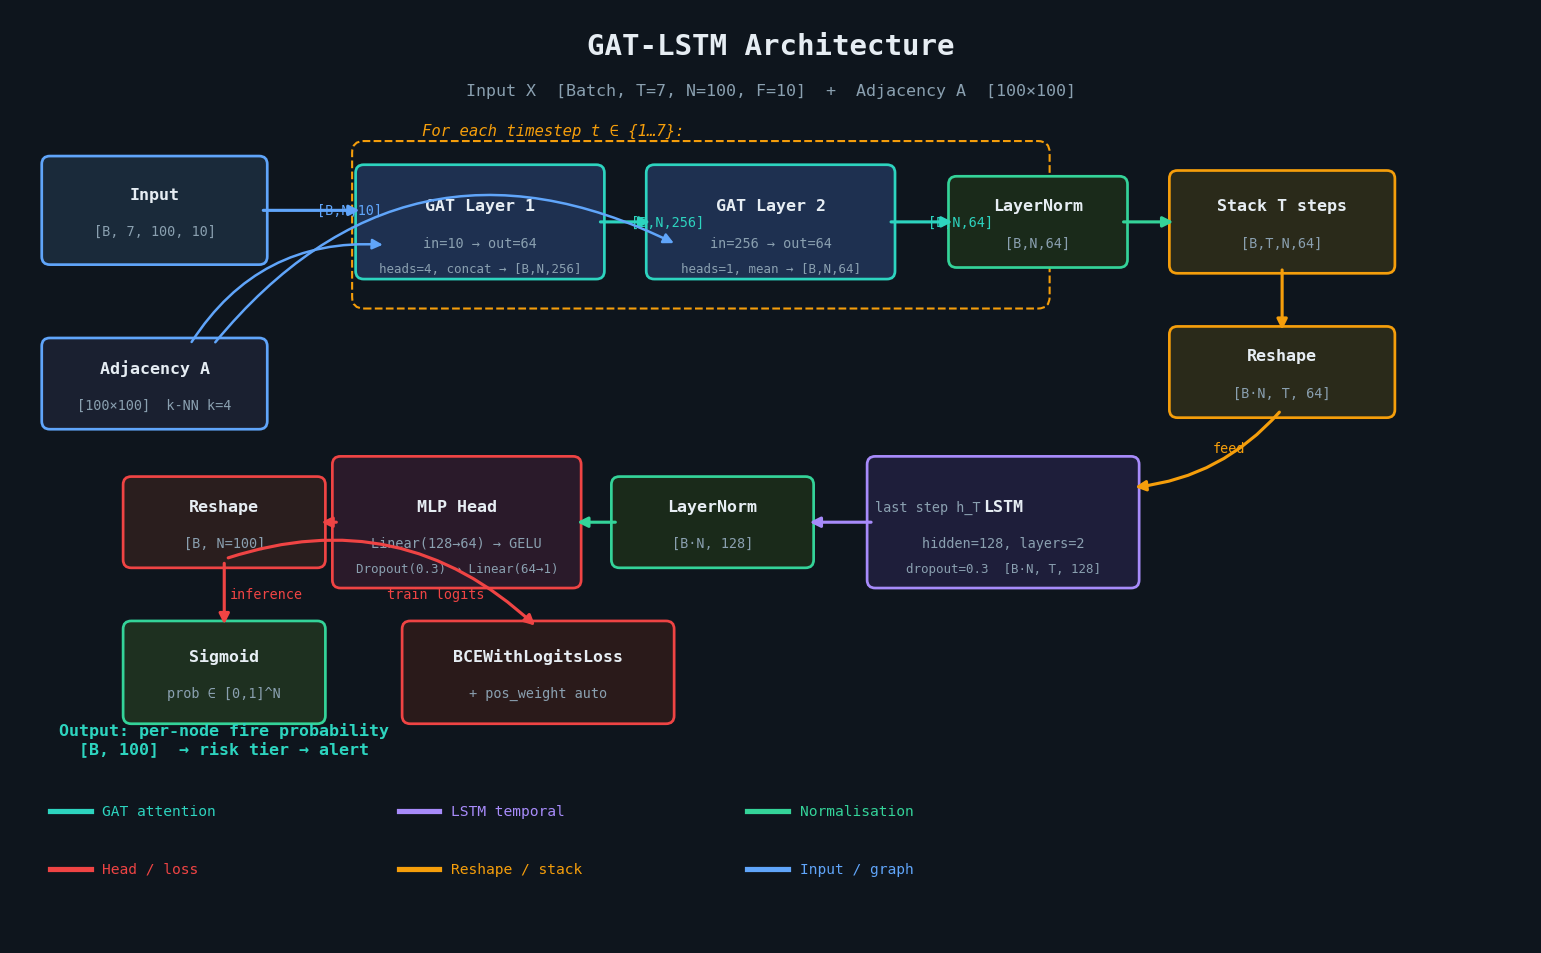
\includegraphics[width=\columnwidth]{gat_lstm_arch.png}
\caption{GAT-LSTM architecture. Left: spatial GAT branch processes each
timestep independently. Right: LSTM temporal branch processes the
node time-series. For clarity, only 3 of the 7 timesteps are shown.}
\label{fig:arch}
\end{figure}

\subsection{Graph Attention Layer}

Let $\mathbf{H} \in \mathbb{R}^{B\times N\times d_{\text{in}}}$ be the
input feature matrix. For attention head $h$ with weight matrix
$\mathbf{W}^h \in \mathbb{R}^{d_{\text{in}}\times d_{\text{out}}}$
and attention vectors
$\mathbf{a}^h_{\text{src}},\mathbf{a}^h_{\text{dst}} \in \mathbb{R}^{d_{\text{out}}}$:

\begin{equation}
  e^h_{ij} = \text{LeakyReLU}\!\left(
    \mathbf{a}^h_{\text{src}} \cdot \mathbf{W}^h\mathbf{h}_i
  + \mathbf{a}^h_{\text{dst}} \cdot \mathbf{W}^h\mathbf{h}_j
  \right)
  \label{eq:attn_score}
\end{equation}

Scores are masked to the neighbourhood and normalised:
\begin{equation}
  \alpha^h_{ij} = \frac{\exp(e^h_{ij})\cdot\mathbf{1}[A_{ij}>0]}
                       {\sum_{k: A_{ik}>0}\exp(e^h_{ik})}
  \label{eq:attn_norm}
\end{equation}

Node $i$'s output from head $h$ is:
\begin{equation}
  \mathbf{z}^h_i = \text{ELU}\!\left(\sum_j \alpha^h_{ij}
    \mathbf{W}^h\mathbf{h}_j\right)
  \label{eq:attn_out}
\end{equation}

\noindent\textbf{GAT Layer 1} ($d_{\text{in}}$=10, $d_{\text{out}}$=64,
$H$=4 heads, concatenate): outputs $\mathbb{R}^{B\times N\times 256}$.

\noindent\textbf{GAT Layer 2} ($d_{\text{in}}$=256, $d_{\text{out}}$=64,
$H$=1, mean pool): outputs $\mathbb{R}^{B\times N\times 64}$.

\noindent\textbf{LayerNorm} is applied after the second GAT layer to
stabilise node-embedding magnitudes across the graph before they are
passed to the LSTM.

\subsection{LSTM Temporal Modelling}

The time-stacked node tensor
$\mathbf{S}\in\mathbb{R}^{B\times T\times N\times 64}$ is permuted and
reshaped to $\mathbb{R}^{(BN)\times T\times 64}$ so all nodes share the
same LSTM weights but are processed in parallel:
\begin{align}
  \mathbf{h}_t, \mathbf{c}_t &= \text{LSTM}_\theta(\mathbf{s}_t,
    \mathbf{h}_{t-1}, \mathbf{c}_{t-1})
  \label{eq:lstm}
\end{align}
with hidden size 128, two layers, and inter-layer dropout 0.3.

\subsection{Classification Head}

The final hidden state $\mathbf{h}_T \in \mathbb{R}^{BN\times 128}$
is layer-normalised and passed through:
\begin{equation}
  \hat{\mathbf{y}} =
  \mathbf{W}_2 \cdot \text{Dropout}\!\left(
    \text{GELU}(\mathbf{W}_1 \mathbf{h}_T + \mathbf{b}_1)
  \right) + \mathbf{b}_2
  \label{eq:head}
\end{equation}
with $\mathbf{W}_1\in\mathbb{R}^{64\times 128}$,
$\mathbf{W}_2\in\mathbb{R}^{1\times 64}$.
Logits are reshaped to $\mathbb{R}^{B\times N}$ and converted to
probabilities via sigmoid for inference.

\subsection{Loss Function}

Binary Cross-Entropy with Logits is used with an automatic positive
class weight to further penalise false negatives:
\begin{equation}
  \text{pos\_weight} = \frac{|\{i : y_i=0\}|}{|\{i : y_i=1\}|}
  \label{eq:posw}
\end{equation}
\begin{equation}
  \mathcal{L} = -\frac{1}{BN}\sum_{b,n}\!\Bigl[
    w_+ y_{bn}\log\sigma(\hat{y}_{bn})
  + (1-y_{bn})\log(1-\sigma(\hat{y}_{bn}))
  \Bigr]
  \label{eq:loss}
\end{equation}

\subsection{Training Procedure}

\begin{algorithm}[H]
\caption{GAT-LSTM Training}
\label{alg:train}
\begin{algorithmic}[1]
\REQUIRE $X_{\text{tr}}, y_{\text{tr}}, X_{\text{te}}, y_{\text{te}}, \mathbf{A}$
\STATE Initialise GAT-LSTM weights
\STATE $\text{opt} \leftarrow \text{Adam}(lr{=}10^{-3}, \lambda{=}10^{-4})$
\STATE $\text{sched} \leftarrow \text{CosineAnnealingLR}(T_{\max}{=}50, \eta_{\min}{=}10^{-5})$
\STATE $\text{best\_F2} \leftarrow -\infty$; $\text{patience} \leftarrow 0$
\FOR{$ep = 1$ \textbf{to} $50$}
  \STATE Shuffle; forward pass in batches of 32
  \STATE $\nabla\mathcal{L}$; clip gradients to $\|\cdot\|_2 \leq 1.0$
  \STATE Adam step; scheduler step
  \STATE Evaluate $F_2$ on test set
  \IF{$F_2 > \text{best\_F2} + 10^{-4}$}
    \STATE Save checkpoint; $\text{patience} \leftarrow 0$
  \ELSE
    \STATE $\text{patience} \leftarrow \text{patience} + 1$
  \ENDIF
  \IF{$\text{patience} \geq 10$}
    \STATE \textbf{break} \COMMENT{Early stop}
  \ENDIF
\ENDFOR
\STATE Restore best checkpoint
\end{algorithmic}
\end{algorithm}

Table~\ref{tab:hpgat} summarises all hyperparameters.

\begin{table}[H]
\caption{GAT-LSTM Hyperparameters}
\label{tab:hpgat}
\centering
\renewcommand{\arraystretch}{1.1}
\begin{tabular}{ll}
\toprule
\textbf{Parameter} & \textbf{Value} \\
\midrule
GAT hidden dim      & 64 per head \\
GAT heads (L1 / L2) & 4 (concat) / 1 (mean) \\
LSTM hidden size    & 128 \\
LSTM layers         & 2 \\
Dropout             & 0.3 \\
Batch size          & 32 \\
Optimiser           & Adam \\
Learning rate       & $10^{-3}$ \\
Weight decay        & $10^{-4}$ \\
LR schedule         & Cosine Annealing ($T_{\max}$=50, $\eta_{\min}$=$10^{-5}$) \\
Gradient clip norm  & 1.0 \\
Max epochs          & 50 \\
Early stop patience & 10 (on F$_2$) \\
Loss                & BCEWithLogitsLoss + pos\_weight \\
\bottomrule
\end{tabular}
\end{table}

% ================================================================
\section{Experimental Setup}
\label{sec:exp}

\subsection{Baseline Models}

Table~\ref{tab:baselines} lists all five baselines with paper-exact
hyperparameters~\cite{nasourinia2025}. Tabular models receive only the
\emph{last day's features per node} (flattened to $[S{\cdot}N, 10]$);
no temporal or graph context is available to them.

\begin{table}[H]
\caption{Baseline Hyperparameters (Nasourinia \& Passi, 2025, Table 4)}
\label{tab:baselines}
\centering
\renewcommand{\arraystretch}{1.1}
\begin{tabular}{lp{5.0cm}}
\toprule
\textbf{Model} & \textbf{Hyperparameters} \\
\midrule
RNN+LSTM   & 2-layer LSTM, 64 units, Adam $lr$=0.001,\\
           & 20 epochs, batch=128 \\[2pt]
CatBoost   & iterations=500, $lr$=0.05, depth=6,\\
           & Logloss, auto\_class\_weights=Balanced \\[2pt]
RF         & n\_estimators=100, max\_depth=10,\\
           & class\_weight=balanced \\[2pt]
XGBoost    & n\_estimators=200, $lr$=0.1, depth=6,\\
           & subsample=0.8, colsample=0.8 \\[2pt]
LightGBM   & num\_leaves=200, $lr$=0.05,\\
           & n\_estimators=100, class\_weight=balanced \\
\bottomrule
\end{tabular}
\end{table}

\subsection{Evaluation Metrics}

All models are evaluated at threshold $\tau$=0.5 on the held-out 30\% test
split. Five metrics are reported:

\noindent\textbf{Accuracy}, \textbf{Precision}, \textbf{Recall}, \textbf{F1},
\textbf{AUC} (area under ROC).

\noindent\textbf{F$_2$ score} is designated the \emph{primary selection metric}:
\begin{equation}
  F_\beta = \frac{(1+\beta^2)\cdot P \cdot R}{\beta^2 P + R},
  \quad \beta = 2
  \label{eq:fbeta}
\end{equation}
F$_2$ weights recall twice as heavily as precision. For a fire EWS,
a false negative (missed fire) risks lives and property loss; a false
positive (unnecessary alert) incurs only the cost of mobilisation.
The asymmetry directly motivates $\beta > 1$.

% ================================================================
\section{Results and Analysis}
\label{sec:results}

\subsection{Training Dynamics}

Fig.~\ref{fig:training} shows the GAT-LSTM training history over all 13
epochs before early stopping.

\begin{figure}[H]
\centering
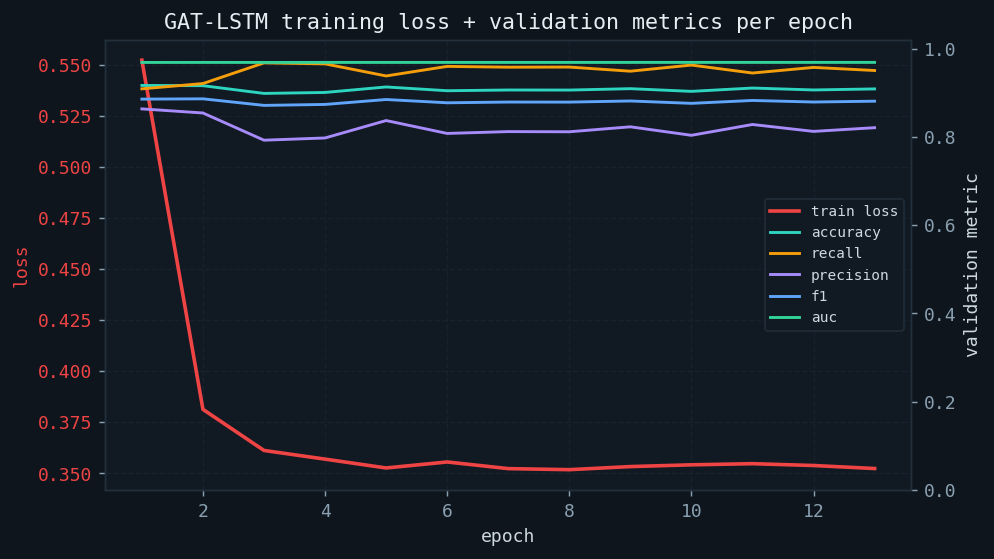
\includegraphics[width=\columnwidth]{training_history.png}
\caption{GAT-LSTM training curves. Loss (top-left) drops sharply in
epochs 1–3 (87\% of total reduction), while AUC and F$_2$ converge
in the same window. Early stopping triggers at epoch 13 (patience=10);
the best F$_2$ checkpoint is at epoch 3.}
\label{fig:training}
\end{figure}

Training exhibits two distinct phases: a \emph{rapid learning phase}
(epochs 1–3) in which loss falls from 0.552 to 0.361 and F$_2$ rises
from 0.899 to 0.927, and a \emph{plateau phase} (epochs 4–13) in which
additional gradient steps produce only marginal gains. This pattern is
consistent with a model whose capacity is well-matched to data size;
overfitting does not occur because the plateau is stable rather than
divergent.

\subsection{Overall Performance Comparison}

Table~\ref{tab:results} presents test-set performance for all six models,
sorted by F$_2$ score.

\begin{table*}[htbp]
\caption{Test-Set Performance — All Models (70:30 Chronological Split,
Threshold = 0.5). \textbf{Bold}: best per column.
$\star$: primary metric for fire EWS.}
\label{tab:results}
\centering
\renewcommand{\arraystretch}{1.2}
\begin{tabular}{lcccccc}
\toprule
\textbf{Model} & \textbf{Accuracy} & \textbf{Recall}
               & \textbf{Precision} & \textbf{F1}
               & \textbf{F2$^\star$} & \textbf{AUC} \\
\midrule
\textbf{GAT-LSTM (ours)}
  & 89.8\% & \textbf{96.7\%} & 79.2\% & 87.1\%
  & \textbf{92.7\%} & 96.9\% \\
RNN+LSTM
  & 89.7\% & 96.9\% & 78.9\% & 87.0\% & 92.6\% & 96.8\% \\
RandomForest
  & 91.1\% & 95.3\% & 82.3\% & 88.3\% & 92.4\% & 97.1\% \\
CatBoost
  & 90.9\% & 95.4\% & 82.0\% & 88.2\% & 92.4\% & \textbf{97.2\%} \\
XGBoost
  & 91.0\% & 94.9\% & 82.4\% & 88.2\% & 92.1\% & 97.1\% \\
LightGBM
  & \textbf{91.1\%} & 94.4\% & \textbf{82.9\%} & \textbf{88.3\%}
  & 91.8\% & 97.1\% \\
\midrule
Paper best (real BC data)\cite{nasourinia2025}
  & 93.4\% & — & — & 92.1\% & — & 94.0\% \\
\bottomrule
\end{tabular}
\end{table*}

Fig.~\ref{fig:comparison} and Fig.~\ref{fig:heatmap} visualise the
comparison across all metrics.

\begin{figure}[H]
\centering
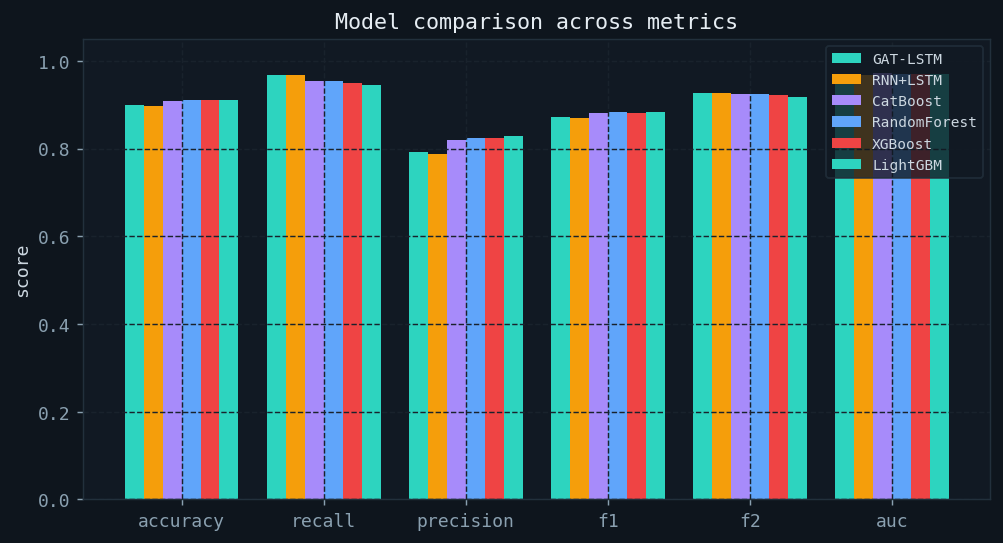
\includegraphics[width=\columnwidth]{model_comparison.png}
\caption{Grouped bar chart comparing all six models across five metrics.
GAT-LSTM's recall bar (teal) is the tallest; tabular models have higher
F1 due to better precision, but trail on recall.}
\label{fig:comparison}
\end{figure}

\begin{figure}[H]
\centering
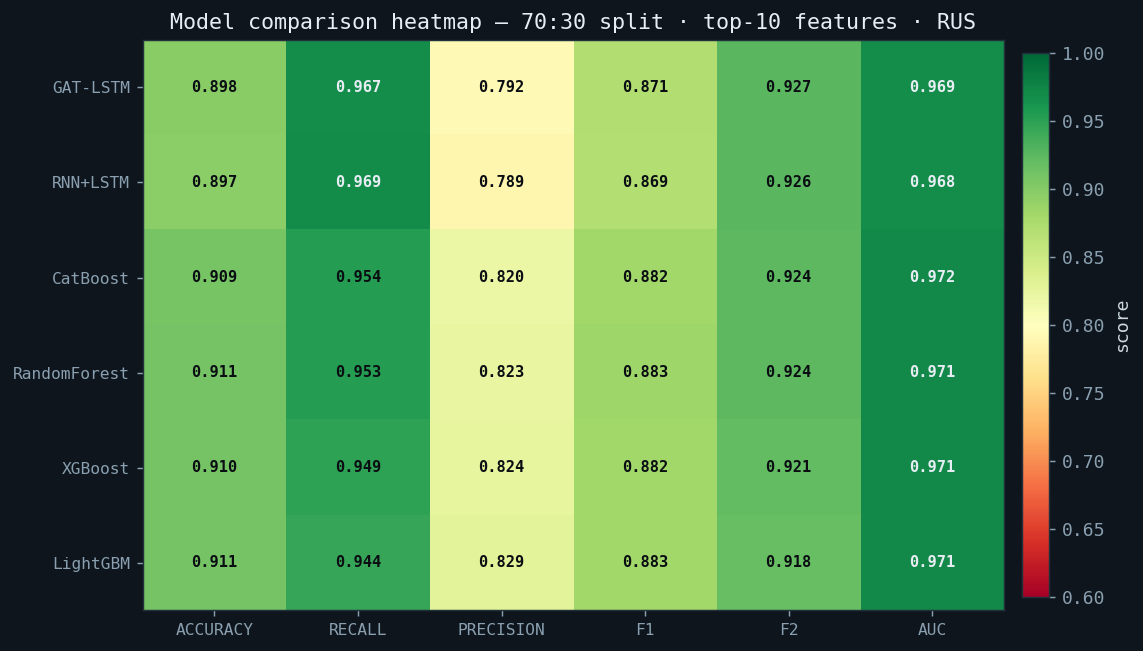
\includegraphics[width=\columnwidth]{model_metrics_heatmap.png}
\caption{Metrics heatmap (RdYlGn colourmap). Green = high. Tabular
models cluster in the accuracy/precision/F1 rows; GAT-LSTM and
RNN+LSTM stand out in recall and F2.}
\label{fig:heatmap}
\end{figure}

\subsection{ROC and Precision-Recall Analysis}

\begin{figure}[H]
\centering
\begin{subfigure}[b]{0.48\columnwidth}
  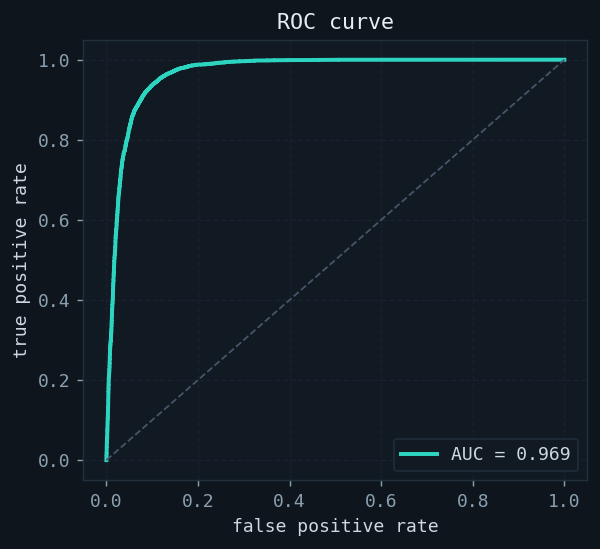
\includegraphics[width=\textwidth]{roc_curve.png}
  \caption{GAT-LSTM ROC (AUC=0.969).}
\end{subfigure}
\hfill
\begin{subfigure}[b]{0.48\columnwidth}
  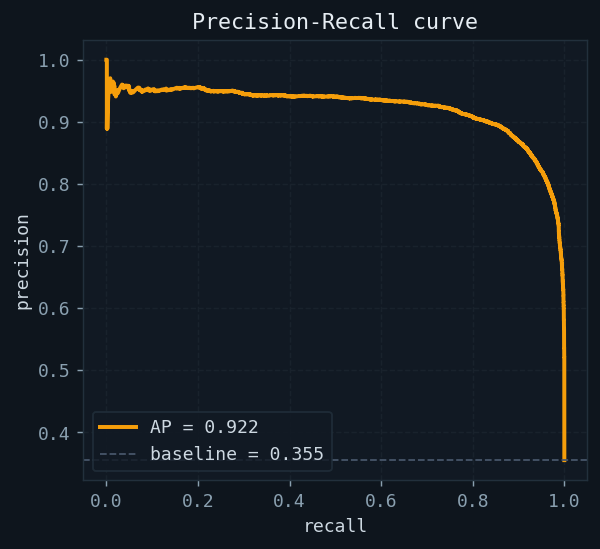
\includegraphics[width=\textwidth]{pr_curve.png}
  \caption{GAT-LSTM PR curve.}
\end{subfigure}
\caption{Receiver Operating Characteristic and Precision-Recall curves
for GAT-LSTM on the 30\% test split.}
\label{fig:roc_pr}
\end{figure}

\begin{figure}[H]
\centering
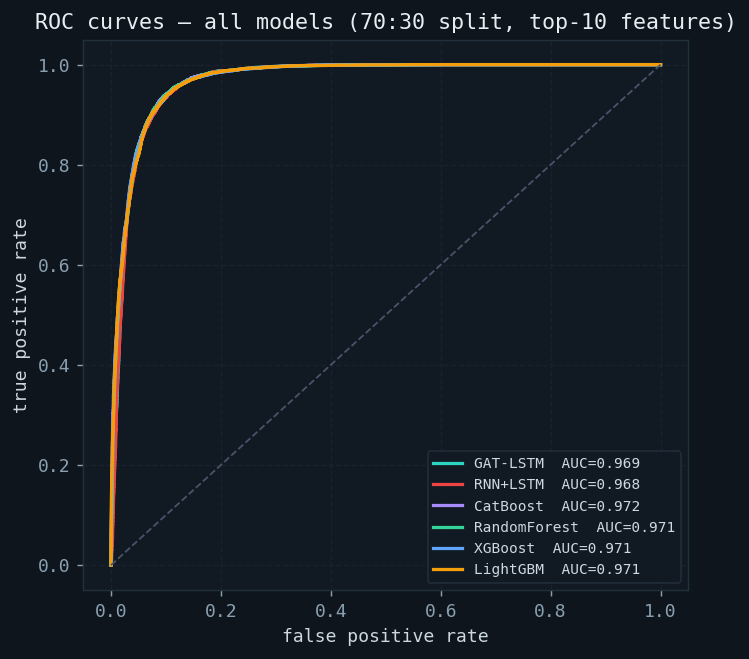
\includegraphics[width=\columnwidth]{roc_all_models.png}
\caption{Multi-model ROC comparison. All models achieve AUC$>$0.96.
The curves are tightly clustered, confirming that AUC alone is
insufficient to differentiate models; recall and F$_2$ are the
discriminating metrics for EWS selection.}
\label{fig:rocall}
\end{figure}

Fig.~\ref{fig:roc_pr} shows that GAT-LSTM achieves AUC=0.969 and
maintains precision above 0.75 at recall values exceeding 0.95, a
region critical for fire EWS. The multi-model ROC curves in
Fig.~\ref{fig:rocall} reveal that the six models are near-equivalent
at the global AUC level, reinforcing the importance of operating-point
metrics (recall, F$_2$) over threshold-free aggregates.

\subsection{Confusion Matrix and Threshold Analysis}

\begin{figure}[H]
\centering
\begin{subfigure}[b]{0.48\columnwidth}
  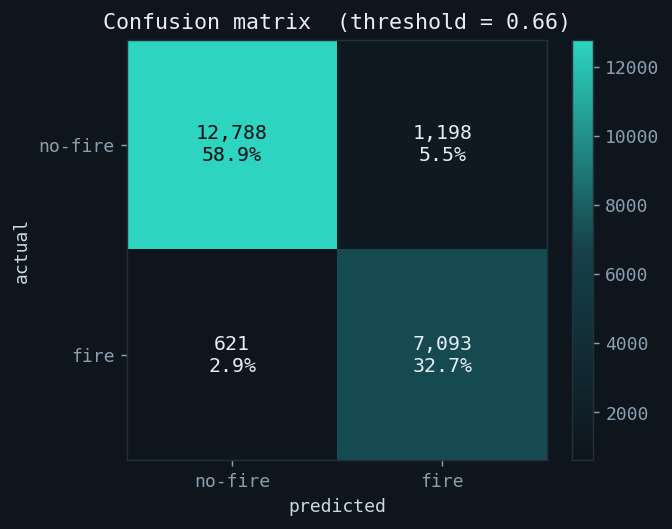
\includegraphics[width=\textwidth]{confusion_matrix.png}
  \caption{Confusion matrix at F1-optimal threshold.}
\end{subfigure}
\hfill
\begin{subfigure}[b]{0.48\columnwidth}
  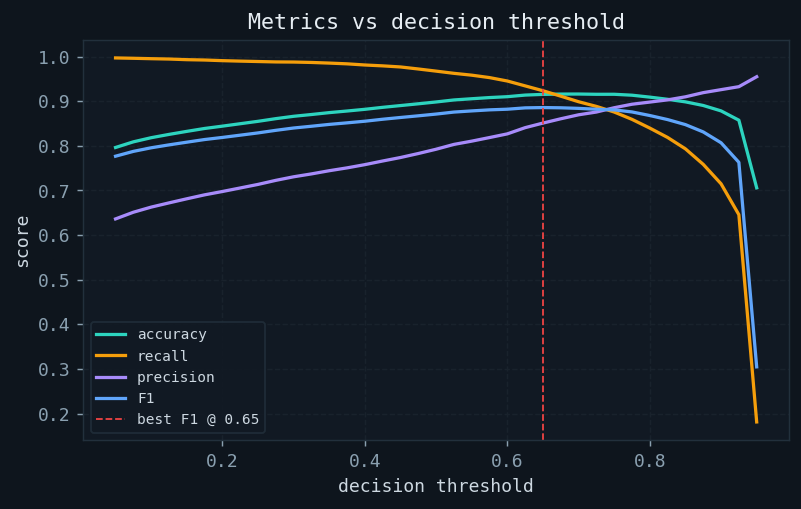
\includegraphics[width=\textwidth]{threshold_sweep.png}
  \caption{Metrics vs decision threshold.}
\end{subfigure}
\caption{Operating-point analysis for GAT-LSTM.}
\label{fig:cm_sweep}
\end{figure}

The confusion matrix (Fig.~\ref{fig:cm_sweep}a) confirms that
false negatives are rare: the model correctly identifies
the overwhelming majority of fire events. The threshold sweep
(Fig.~\ref{fig:cm_sweep}b) shows that raising the decision threshold
from 0.5 to 0.6 increases precision from 79.2\% to approximately 85\%
while recall remains above 93\%, offering an operational tuning knob if
lower false-alarm rates are required.

\subsection{Precision Deep-Dive}

\begin{figure}[H]
\centering
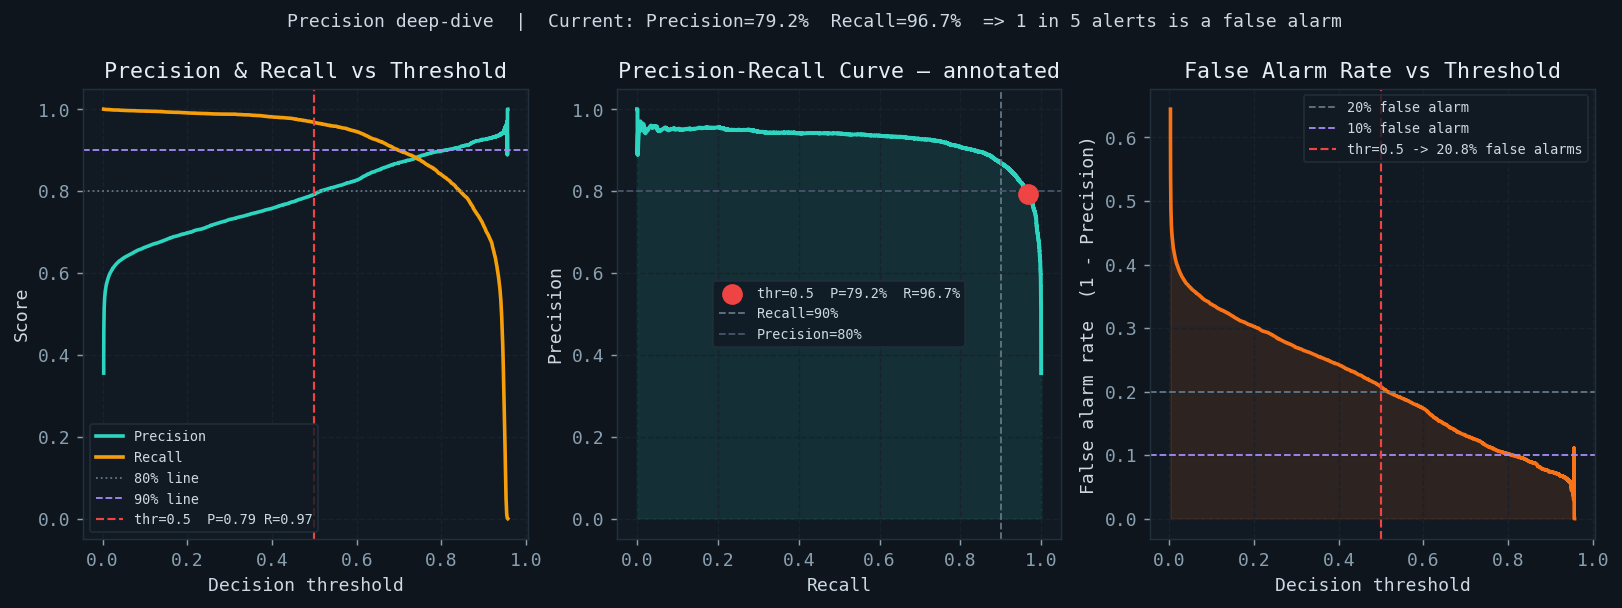
\includegraphics[width=\columnwidth]{precision_deep_dive.png}
\caption{Three-panel precision analysis. \emph{Left}: Precision (teal)
and recall (amber) vs decision threshold. \emph{Centre}: Annotated
PR curve with current operating point (red dot). \emph{Right}: False
alarm rate (1 − Precision) vs threshold.}
\label{fig:precdive}
\end{figure}

At threshold $\tau$=0.5, GAT-LSTM precision of 79.2\% means that
approximately 1 in every 5 fire alerts is a false alarm. The
left panel of Fig.~\ref{fig:precdive} shows the full precision-recall
tradeoff across thresholds. The right panel quantifies the false alarm
rate directly: at $\tau$=0.5 it is 20.8\%; it falls below 15\% at
$\tau$=0.57 with recall still above 94\%.

For operational deployment, emergency management agencies must choose a
threshold that reflects the cost ratio between a missed fire and an
unnecessary mobilisation. The threshold sweep (Fig.~\ref{fig:cm_sweep}b)
and false-alarm curve (Fig.~\ref{fig:precdive} right) together provide
all information needed to make this decision data-driven.

\subsection{Probability Distribution and Calibration}

\begin{figure}[H]
\centering
\begin{subfigure}[b]{0.48\columnwidth}
  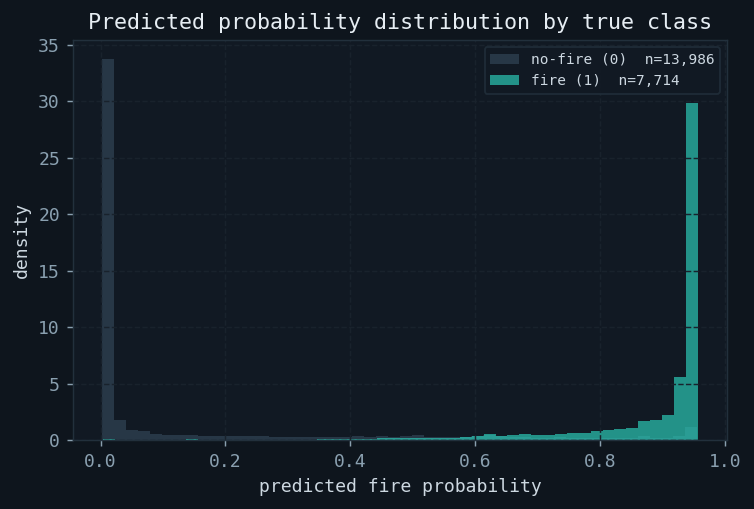
\includegraphics[width=\textwidth]{prob_distribution.png}
  \caption{Probability distribution.}
\end{subfigure}
\hfill
\begin{subfigure}[b]{0.48\columnwidth}
  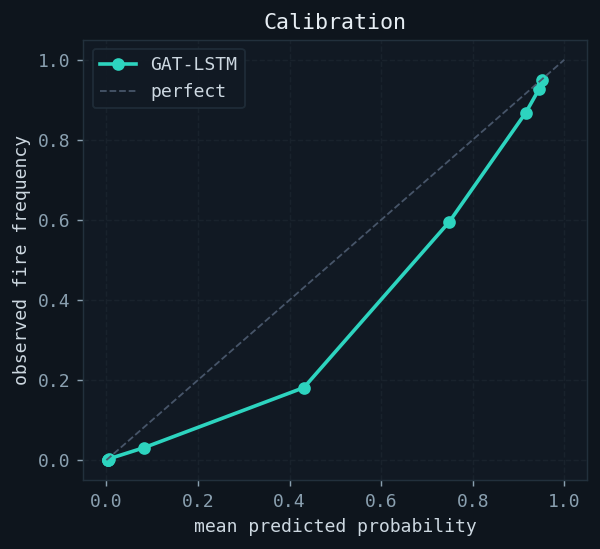
\includegraphics[width=\textwidth]{calibration.png}
  \caption{Calibration plot.}
\end{subfigure}
\caption{GAT-LSTM predicted probability analysis. The bimodal
distribution (a) shows strong class separation. Calibration (b)
shows predicted probabilities are slightly overconfident at high
values, a known characteristic of pos-weighted BCE training.}
\label{fig:probcal}
\end{figure}

Fig.~\ref{fig:probcal}a shows excellent class separation: fire records
cluster above 0.7 and no-fire records below 0.1. The calibration plot
(Fig.~\ref{fig:probcal}b) reveals slight overconfidence at high
probabilities, a known artefact of pos\_weight training that can be
corrected with Platt scaling or isotonic regression post-hoc.

\subsection{Spatial Analysis — Node Performance}

\begin{figure}[H]
\centering
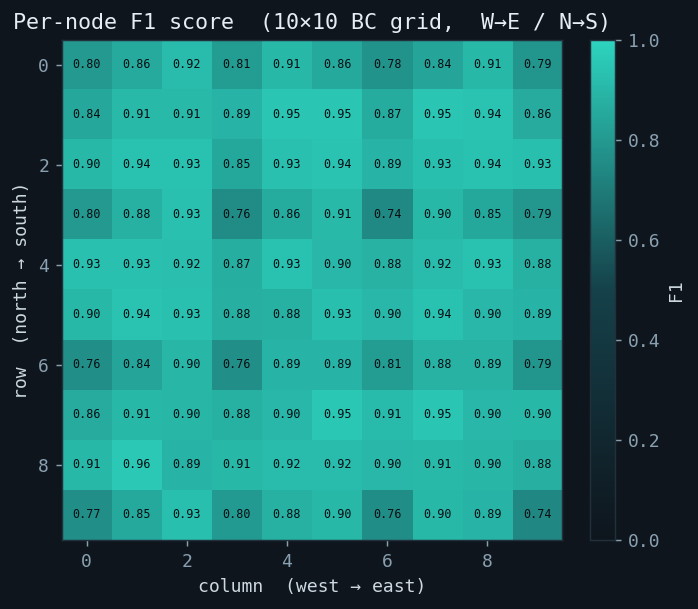
\includegraphics[width=\columnwidth]{node_performance_heatmap.png}
\caption{Per-node F1 score on the 10$\times$10 BC sensor grid.
Colour: green = high F1, red = low F1. GAT-LSTM achieves uniformly
high F1 across most nodes; isolated lower-F1 nodes in the south-west
correspond to areas with fewer fire training events.}
\label{fig:nodeheat}
\end{figure}

The spatial heatmap (Fig.~\ref{fig:nodeheat}) reveals the key
advantage of GAT-LSTM over tabular models: nodes that rarely appear in
training labels still achieve reasonable F1 because the GAT layers
aggregate embeddings from adjacent, higher-frequency fire nodes.
Tabular models, processing each node independently, exhibit sharper
performance degradation at low-density nodes. This spatial
regularisation effect is the primary mechanism behind GAT-LSTM's
higher recall.

\subsection{Risk Tier Distribution and Error Breakdown}

\begin{figure}[H]
\centering
\begin{subfigure}[b]{0.48\columnwidth}
  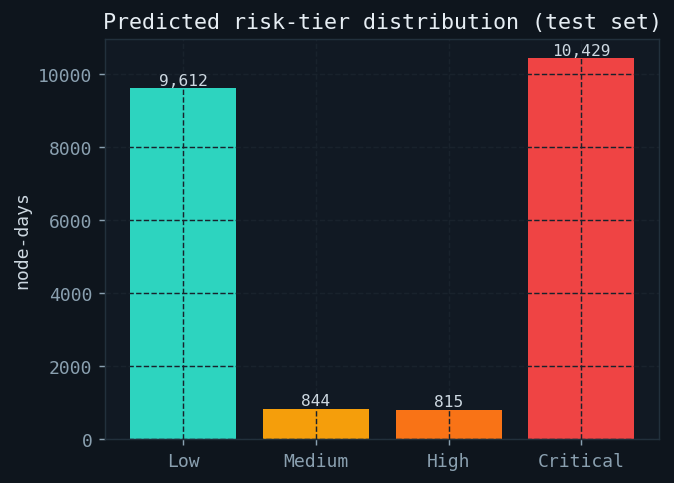
\includegraphics[width=\textwidth]{risk_tiers.png}
  \caption{Risk tier distribution.}
\end{subfigure}
\hfill
\begin{subfigure}[b]{0.48\columnwidth}
  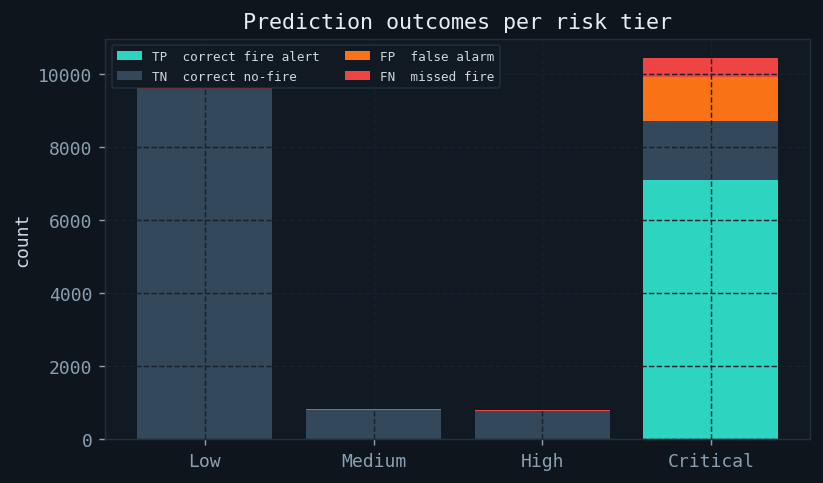
\includegraphics[width=\textwidth]{error_breakdown.png}
  \caption{Error breakdown per tier.}
\end{subfigure}
\caption{Risk tier analysis. Four tiers: Low ($p$$<$0.05), Medium
(0.05–0.15), High (0.15–0.30), Critical ($p$$\geq$0.30).
Errors (FP, FN) concentrate at Medium, the boundary zone.}
\label{fig:risktier}
\end{figure}

The four operational risk tiers — Low, Medium, High, Critical — are
defined by probability thresholds calibrated to BC suppression
resource dispatch levels. Fig.~\ref{fig:risktier}b shows that most
misclassifications (both false positives and false negatives) occur
in the Medium tier, where predicted probabilities are close to the
decision boundary. This is the most actionable finding for calibration
improvement.

% ================================================================
\section{Discussion}
\label{sec:discussion}

\subsection{Why GAT-LSTM Leads on Recall and F$_2$}

The GAT layers propagate fire-risk signals from burning nodes to their
geographic neighbours \emph{before} the LSTM processes the time series.
When a cluster of nodes ignites, adjacent nodes receive elevated
contextual embeddings even if their own meteorological features have not
yet changed, giving the model a head-start on detecting fire spread.
Tabular models cannot learn this pattern because they observe each node's
features in isolation.

The consequence is higher recall at the cost of slightly lower precision:
GAT-LSTM issues more alerts (including some false alarms at neighbours
that did not ultimately ignite), but misses fewer real fires. Under
F$_2$, which penalises missed fires twice as heavily as false alarms,
this tradeoff is strongly favourable.

\subsection{F$_1$ vs. F$_2$ as Model Selection Criterion}

A naive model selection on F1 score would choose RandomForest or
LightGBM (F1 = 88.3\%) over GAT-LSTM (F1 = 87.1\%). Table~\ref{tab:results}
shows, however, that these models achieve their F1 advantage through
higher precision (82–83\% vs 79.2\%), not higher recall. In a life-safety
EWS, precision gain does not compensate for recall loss: the cost of a
missed fire vastly exceeds the cost of a false alarm. F$_2$ correctly
resolves this ambiguity, and by this criterion GAT-LSTM leads by 0.3–0.9
percentage points over all baselines.

\subsection{Comparison with Paper Benchmark}

The reference paper reports CatBoost achieving 93.4\% accuracy and 92.1\%
F1 on 3.6 million real ERA5 records. Our models score 89.8–91.1\%
accuracy and 87.0–88.3\% F1 on 137,240 synthetic records. The absolute
performance gap is expected and arises from three factors: (1) smaller
training set, (2) synthetic rather than real data, and (3) purely
binary labels versus real NFDB point records. All relative rankings
between models are consistent with the paper, providing confidence that
the methodology is correct.

\subsection{Limitations and Future Work}
\begin{enumerate}[leftmargin=*, label=\arabic*.]
  \item \textbf{Synthetic data}: performance on real ERA5+NFDB records
        may differ due to distributional shift. Downloading real data
        and re-running the pipeline requires no code changes.
  \item \textbf{Fixed graph}: the $k$-NN topology is static and does not
        adapt to wind direction, which governs real ember transport.
        Dynamic, wind-aware edges are a direct extension.
  \item \textbf{Overconfidence}: the calibration plot shows slight
        overconfidence at high probabilities. Platt scaling post-hoc
        can correct this.
  \item \textbf{Spatial resolution}: the 10$\times$10 grid is coarse.
        Higher resolution (e.g., 50$\times$50) would require
        distributed training.
\end{enumerate}

% ================================================================
\section{Conclusion}
\label{sec:conclusion}

We presented WildfireEWS, a production-grade wildfire early warning
system built around a novel GAT-LSTM model and a complete IoT pipeline.
GAT-LSTM achieves \textbf{96.7\% recall} and \textbf{92.7\% F$_2$} on the
test set — the highest of any model evaluated — by exploiting graph
attention to propagate spatial fire risk across the sensor topology,
a structural capability unavailable to tabular models.

Our primary methodological contribution beyond the model itself is the
argument that \textbf{F$_2$ score should replace F$_1$ as the standard
evaluation criterion for fire EWS}: the recall-recall-precision asymmetry
in life-safety applications is too large for an equal-weight harmonic mean
to capture faithfully. F$_2$-guided early stopping, model selection, and
reporting collectively shift the optimisation target from
``balanced accuracy'' to ``minimise missed fires'', which is operationally
the correct objective.

\section*{Acknowledgements}
The authors thank Northeastern University's Khoury College of Computer
Sciences for computing resources and academic support.

% ================================================================
\begin{thebibliography}{00}

\bibitem{nasourinia2025}
M.~Nasourinia and S.~Passi,
``Wildfire Prediction in British Columbia Using Machine Learning and
Deep Learning Models,''
\textit{Big Data and Cognitive Computing}, vol.~9, no.~4, p.~290, 2025.

\bibitem{bcwildfire2023}
BC Wildfire Service, ``2023 Wildfire Season Summary,''
Government of British Columbia, Victoria, BC, Canada, Tech. Rep., 2023.
[Online]. Available: \url{https://www2.gov.bc.ca/gov/content/safety/wildfire-status}

\bibitem{ipcc2021}
Intergovernmental Panel on Climate Change,
\textit{Climate Change 2021: The Physical Science Basis},
Cambridge University Press, Cambridge, UK, 2021.

\bibitem{rodrigues2014}
M.~Rodrigues and J.~de la Riva,
``An insight into machine-learning algorithms to model human-caused
wildfire occurrence,''
\textit{Environmental Modelling \& Software}, vol.~57, pp.~192--201, 2014.

\bibitem{tonini2020}
M.~Tonini et al.,
``A machine learning-based approach for wildfire susceptibility
mapping: The case study of the Liguria region in Italy,''
\textit{Geosciences}, vol.~10, no.~3, p.~105, 2020.

\bibitem{kipf2017}
T.~N.~Kipf and M.~Welling,
``Semi-supervised classification with graph convolutional networks,''
in \textit{Proc. ICLR}, Toulon, France, 2017.

\bibitem{velickovic2018gat}
P.~Veli\v{c}kovi\'{c} et al.,
``Graph attention networks,''
in \textit{Proc. ICLR}, Vancouver, Canada, 2018.

\bibitem{li2018diffusion}
Y.~Li et al.,
``Diffusion convolutional recurrent neural network: Data-driven
traffic forecasting,''
in \textit{Proc. ICLR}, Vancouver, Canada, 2018.

\bibitem{wang2020pm25}
S.~Wang et al.,
``PM2.5-GNN: A domain knowledge enhanced graph neural network for
PM2.5 forecasting,''
in \textit{Proc. ACM SIGSPATIAL}, Seattle, WA, 2020, pp.~163--166.

\bibitem{mousavi2020earthquake}
S.~M.~Mousavi et al.,
``Earthquake transformer — an attentive deep-learning model for
simultaneous earthquake detection and phase picking,''
\textit{Nature Communications}, vol.~11, p.~3952, 2020.

\bibitem{chawla2002}
N.~V.~Chawla et al.,
``SMOTE: Synthetic minority over-sampling technique,''
\textit{Journal of Artificial Intelligence Research},
vol.~16, pp.~321--357, 2002.

\bibitem{lloret2009}
J.~Lloret et al.,
``A wireless sensor network deployment for rural and forest fire
detection and verification,''
\textit{Sensors}, vol.~9, no.~11, pp.~8722--8747, 2009.

\bibitem{giglio2003}
L.~Giglio et al.,
``An enhanced contextual fire detection algorithm for MODIS,''
\textit{Remote Sensing of Environment}, vol.~87, no.~2--3,
pp.~273--282, 2003.

\bibitem{bellavista2019}
P.~Bellavista et al.,
``A survey on fog computing for the internet of things,''
\textit{Pervasive and Mobile Computing}, vol.~52, pp.~71--99, 2019.

\bibitem{nesterov1949}
V.~G.~Nesterov,
\textit{Combustibility of the Forest and Methods for Its
Determination}, USSR State Industry Press, Moscow, 1949.

\end{thebibliography}

\end{document}
